\documentclass[norsk,a4paper,12pt]{article}
\usepackage{graphicx}
\usepackage[utf8]{inputenc}
\graphicspath{ {Bilder/} }
\usepackage{hyperref}
\usepackage{commath}
\usepackage{float}
\usepackage{mathtools}


\usepackage[T1]{fontenc}
\begin{document}
\title{Linær regresjoni}
\author{Eirik vetle Winnness}
\maketitle 

\section*{Abstract}
I dnne oppgaven eller eksprimtet skal jeg se på hvordan vi kan bruk linære reggresjon til å lage en model som kan tilsån at vi kan bruke tilgere data til å gjenskape en funksjon. Fungerer dettte?. Slik resultane viser greier vi og oppnå noe lik form, men ikke eksakte like verdier som funksjonen selv har. 
\section*{Introduction}
I dette prosjektett skal jeg se på hvordan de tre forjellig mtodene OLS, ridge, og Lasso best greier å etterligne den ekte fuksjonen(Frankfuksjon). Linær regresjon er en metode man kan bruke for å kunne spå hvordan ny data vil oppføreseg, basert på gammel data. Jeg skal studere MSE(), R2, Bias, og. Jeg har skal studere random data ved å genere det i python programmet ankonda og dens pakker. Jeg skal så se på de fire faktorene og studere OLS, ridge og Laso: Hvilen algorytme er det som greier å gi best resultat. Om noen de metodene er bedre til å etterligne datan. jeg kommer til å bruke trenings data for å lage en model, så ser jeg om denne modellen tilppaser seg godt opp mot den virklig fuksjonen. 
\\
I a,b og cbruker jeg k-fold for å splitte opp dataen i trening og test sett. Jeg splitter 1000 datapungter inn i ti deler. Et test data sett, og 9 andre treningset. Når jeg analyser OLS ser jeg på de forsjellige treningsettene, mens i rige og lasso tar jeg gjenommsnitte verdien (mse, r2, bias, var), for se hvordan de oppfører seg i de forsjelige graden $x^g$.
\\
Det blir litt anderledes når jeg ser på faktisk ekte data da velger jeg en del av et ommråde i dataen. Jeg lager en model som produserer en   $\beta$.jeg bruker en trenings verdi og en test verdi for $\hat{X}$. Nå som vi ikke har en funskjon då må vi bruke daten fra terenget som funksjonen. Hvor godt er det denne $\beta$-en greier å gjenskp den virklige Z ($y = X\beta$). dettet gjør jeg med 5 deler fra dataen. Deter er veldig tungt å gjøre dette det er derfor jeg ikke bruker så mange forsjellige treningsett. men velger heller å bruke det forsjellige z(ommeråder) funksjonen. også varierer jeg gradene med(4-11)etter som jeg har set på verien og funnet ut av at dette er det ommrådet som gir greierst verdier(serlig r2) . håper ikke jeg har misforstått oppgaven.
\\
Det tok lit tid før jeg før jeg skjønte at jeg skulle brukke den dataen vi lastet ned  eller den dere ga oss verdiene til en funksjon.
\section*{Teori}
\subsection*{MSE}
MSE = Mean squard error
\[ MSE(y,\hat{\widetilde{ y}}) =\frac{1}{n}\sum^{n-1}_{i=0}(y_i -\widetilde{ y_i})^2\]


\[ MSE = Bias^2 + var(x)\]
\subsection*{R2}

\[ R2(y,\hat{\widetilde{ y}}) =1-\frac{\sum^{n-1}_{i=0}(y_i -\widetilde{ y_i})^2}{\sum^{n-1}_{i=0}(y_i - \bar{y_i})^2} \]
Gjennomsnittet av $\hat{y}$ er definert som:\[\bar{y} =\frac{1}{n}\sum^{n-1}_{i=0}(y_i)\]
\[\bar{y} =\frac{1}{n}\sum^{n-1}_{i=0}(y_i)\]

\subsection*{variancei}
Varians kan bli sett på som  hvordan et sett av random variabler er varierer i forhold til gjenommsnittet.
\[var(x)= \bar{(x^{2})}-(\bar{x})^{2}\]

\subsection*{Bias}





\[bias^{2} =(\frac{1}{n}\sum_{i=1}^{n}{(y-\bar{y_{Spåd}})^{2}})^2\]



\subsection*{ Ordinary Least squar}
		\[\hat{y} = \hat{X}\beta+ e\]
		\[\hat{\beta} =(\hat{X}^{T}\hat{X})^{-1}\bar{X^T}\bar{y}\]


\subsection*{ Ridge Regression}
Leas absoulte shrinkage and select operator
	\[h(b_0,b-1,...,b_k)=\sum^{n}_{i=1}[Y_i -(b_0,b_{1}x_{i1},...,b_{k}x_{ik})]^2 + \lambda \sum_{j=1}^{i}\abs{b_{j}^2}\]
	\[\lambda=Til-pasnings-verdi= konstant\]
	\[\hat{I}=Identitets matris \]
	\[\hat{\beta} =[\hat{X}^{T}\hat{X}+ \lambda \hat{I}]^{-1}\hat{X^T}\hat{y}\]


\subsection*{Lasso Regression}
Leas absoulte shrinkage and select operator
\[h(b_0,b-1,...,b_k)=\sum^{n}_{i=1}[Y_i -(b_0,b_{1}x_{i1},...,b_{k}x_{ik})]^2 + \lambda \sum_{j=1}^{i}\abs{b_j}\]
Går ikke inn på denne teorien for den er ganske kompliset. I mine forsøk har jeg brukt sklearn.linear model linære model

\subsection*{K-fold}
K-fold er en måte for å teste dataen model man har laget på data som man ikke har brukt  for å lage moddel. Da splitter man dataen man har har opp i en hvis mengde deler. jeg splittet opp i 10 deler. Lot et sett være test data. Og lagde 9 andre forsjellige treningss data. Men fant ut sener at man skulle gjøre omvent. At det nemlig var sån at man skulle lage en model  og ha stor andel test data. 
\section*{ Ordinary Least squar}
\begin{figure}[H]
\includegraphics[width=100mm]{olsA_plot}
\caption{3d plot. Det til vestre er spådde daen figur av grad 5. Figuren til høyre er ekte funksjonen}
\end{figure}
\begin{figure}[H]
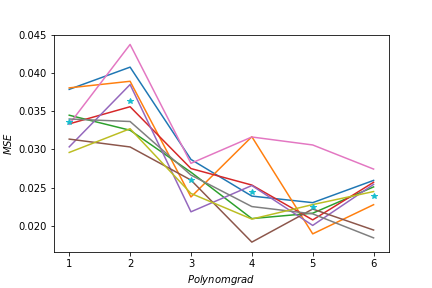
\includegraphics[width=100mm]{MSE}
\caption{Her ser vi de forsjellige trenings datane MSE for de forsjelige gradene 1 til 6($x^g,y^g$). Der de b lyseblåe stjernene er gjennomsnitte av grad 1,2,...,6  }
\end{figure}
På figur over ser vi de forjellige verdien til MSE og gjenoomsnit verdien til de forsjelige treninges daten. vi kan se at vi har en veldig høy verdi for MSE, men den blir lavere etter hvert som høyere grader av x og y blir lagt til i $\hat{X}$. Vii ser også at vi fåren en liten stigning fra grad 5 til 6. Det kan hend at  MSE blir værre om vi legger til høyere grader av x og y. Vi skal ha en MSE verdi som er nærmest null. Gjennomsnitverdien er cirka 0.225 no som er ganske høyt.

\begin{figure}[H]
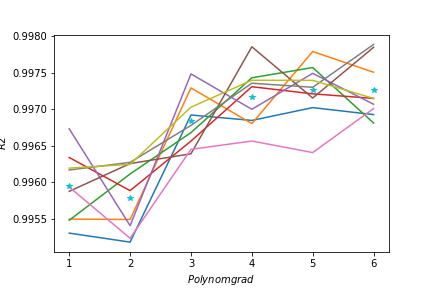
\includegraphics[width=100mm]{R2}
\caption{På denne figuren ser vi R2 skoren. Med trenings daten og gjennomsnite verdien(blå stjerne) }
\end{figure}
Som forventet ser vi at R2 scoren blir bedre desto større graden på x og y. Scoren er ikke noe å skryte av, siden scoren skal være nermest 1 som mulig. Og på figur 3 ser vi at flater ut ved 0.74(grad 5, og 6)



\begin{figure}[H]
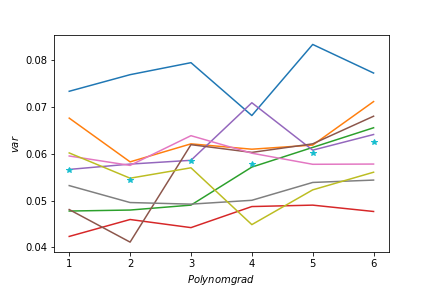
\includegraphics[width=100mm]{var}
\caption{Her ser vi Variansen, for de forsjelige gradene 1 til 6($x^g,y^g$) og gjennomsnits verdien  }
\end{figure}

Ser at variansen holder seg lav. Det er bra at variansen er posetiv. Og at variansen lav betyr at datan ikke varier så mye fra gjennomsnitte 

\begin{figure}[H]
\includegraphics[width=100mm]{Bias}
\caption{ Her ser vi $Bias^2$, for de forsjelige gradene 1 til 6($x^g,y^g$) og gjennomsnits verdien }
\end{figure}

$Bias^2$ holder seg ganske likt over allle gradene. Bias er jo summen av  forjellen den spåddegjennomsnitt  verdien minus den ekte verdien min, delt på antalle verdier. Jeg ville jo tro att denne verdien ville synke voldsomt etter at man næremer seg den ekte y-verdien. 
\subsection*{Diskusjon}
Vi vet at $MSE = Bias^2 + var$. Ut ifra grafene kan vi se at dette ikke stemmer med min data. Noe jeg synes er veldig rart. MSE og r2 har  greier verdier. hvia vi ser på 3d bilde så ser vi at den har samme form som og ligner mye på den ekte funksjonen



\section*{ Ridge Regression}
\begin{figure}[H]
\includegraphics[width=100mm]{r_plot}
\caption{Her ser vi 3D plot av frankfunskjsijone med støy normalt fordelt. }
\end{figure}
l

\begin{figure}[H]
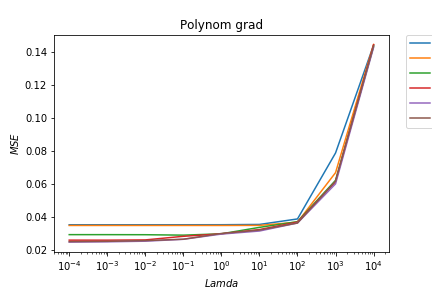
\includegraphics[width=100mm]{MSE(R)}
\caption{MSE vs log($\lambda$), Gradene varier fra 1-6}
\end{figure}
Hvis vi ser på figure 7 kan vi se at jo høyer lamda verdier $\lambda$ blir MSE verdiene høyere.Ser også at det er grad 5 og 6 som  gjelder. Den halverer MSE scoren.

\begin{figure}[H]
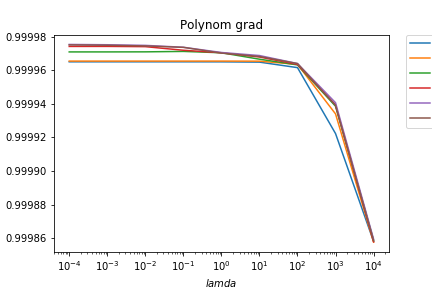
\includegraphics[width=100mm]{r2(R)}
\caption{R2 vs log($\lambda$), Gradene varier fra 1-6  }
\end{figure}
R2 scoren oppfører seg gnskel likt so med MSE figur(8). Høye $\lambda$ gir dårlig R2 score. Viser også at det er grad 5-6 som gir best resultat
\begin{figure}[H]
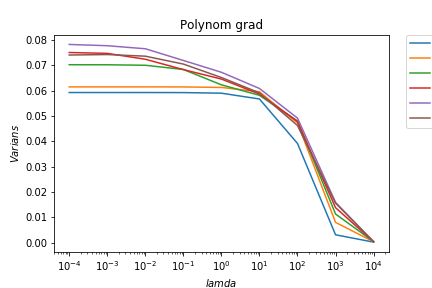
\includegraphics[width=100mm]{var(R)}
\caption{var vs log($\lambda$), Gradene varier fra 1-6 }
\end{figure}
På figur 9 kan vi se variancen for Rige. Den holder seg posetiv som er bra. Og veridene er veldige lave, noe som igjen tydeer på at verdien ikke varerer serlig fra gjennomsnittet. Noe som er veldig interesangt er at jo større $\lambda$ blir mindre blir variangsen. Dette betyr kansje $\beta$-ene blir så store at de jevner ut Z . Hvis alle Z like vil jo variansen være null. 
\begin{figure}[H]
\includegraphics[width=100mm]{Bias(R)}
\caption{$Bias^2$ vs log($\lambda$), Gradene varier fra 1-6 }
Bias holder seg meget la intill  $\lambda = 10^3$ 


\end{figure}


\subsection*{Diskusjon Rige}

Her ser vi også at $MSE = Bias^2 + var(x)$ ikke holder. MSE holder seg meget lav rundt $0.003$, mens varians ligger på $0.008 $ og  $bias ^2=0.0009$ spørmålet her er jo at varians er 8 ganger større enn biasen. Dette tyder på at algorytmen overfitter. jeg har jo lagt normalfordelt støy på $0.1\times støy$. hvis støy blir for stor vil man fitte mer etter denne enn  selve  de faktiske verdien.


\section*{Lasso Regression}
\begin{figure}[H]
\includegraphics[width=100mm]{las_plot}
\caption{MSE vs log($\lambda$), Grad varier fra 5.  }
\end{figure}
Vi ser på fiur 11 att 3d plottet til Lasso ikke følger helt formen til den ekte overflaten. Vi kan se med en gang at det er en forsjell.
\begin{figure}[H]
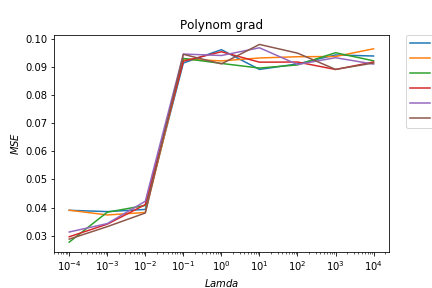
\includegraphics[width=100mm]{MSE(L)}
\caption{MSE vs log($\lambda$), Gradene varier fra 1-6 }
\end{figure}
Vi ser her også hvordan verdien er avhengig av $\lambda$. Svært små $\lambda$ gir svært  gode MSE verdier. Greie.Mello, $10^{-2} $ og $10^{-1}$ skjer det noe da får vi en svært hopp i MSE verdier fra rundt 0,03 til 0,09. 0,09 er jo fremdeles en veldig go skår 

\begin{figure}[H]
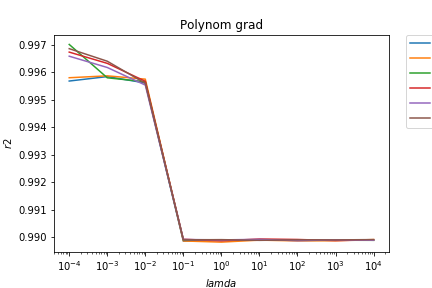
\includegraphics[width=100mm]{r2(L)}
\caption{R2 vs log($\lambda$), Gradene varier fra 1-6}
\end{figure}
R2 skåren til lasso kan vi sse på figur 13. Lasso har aksepable verdier intil $\lambda = 10^{-1}$. En skår mellom 0.7 og 0.6 er helt ok verdier.
\begin{figure}[H]
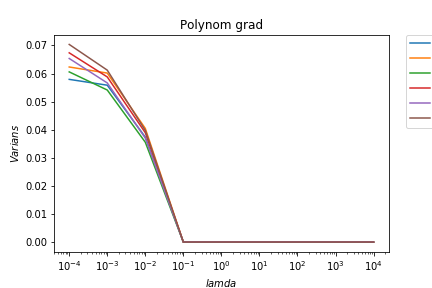
\includegraphics[width=100mm]{var(L)}
\caption{var vs log($\lambda$), Gradene varier fra 1-6 }
\end{figure}
Variansen(figur 14) følger r2 scorens mønster ved at den gpr fa akseptable verdier til ikke akseptable verdier fra$\lambda 10^{-1}$
\begin{figure}[H]
\includegraphics[width=100mm]{Bias(L)}
\caption{$Bias^2$ vs log($\lambda$), Gradene varier fra 1-6 }
Bias for lasso på figur 15 følger også mønstret til var og r2. Den endrer seg ved $10^{-1}$,men den er lavest ved $[10^{-3},10^{-2}]$. Den har en overaskende oppførsel etter som gradene ikke nødvedighvis har den lavest biasen. men nå betyr ikke det at den lavste bias er den beste tilpasningen.
\end{figure}
\subsection*{diskusjon Lasso}
Som vi ser så er ikke 3d projeksjonen noe serlig bra. den følger foren. men det virker som detaljen ike følger. Her har vi også noe som ligner å være en underfitt etter som variansen er mye større en bias. $MSE\neq bias^{2} + var $. Mulig jeg har gjort noe feil med lignigene?? Siden dette gjentar seg.
\subsection*{Diskusjon OLS vs Rige vs LASSO}
Fra både verdier og grafisk 3d fremstiling, Så kommer Rige for meg klart på topp MSE og R2 verdier som ligger på 0.003 og 0.8. Er mye bedre enn hva OLS og LASSO kommer med. Rige er også mindre følsom når det kommer $\lambda$ sine verdier. Selv om Rige har en laver $bias^2$ så virker ikke det som at det gjør at den legger mer merke til støyen. Ser nesten ut som det er lasso som blir mer påvirket av støyen. etter den får noe høyere på verdier på grafen. helt opp mot 1. Hvis jeg plotter lasso grad 10 så begyner den å nærme seg formen som Rige og ols klare og etterligne.

\section*{Real data}
\begin{figure}[H]
\includegraphics[width=100mm]{plot}
\caption{OLSE, grad 11, utrag 300$\times$150 }
\end{figure}
\begin{figure}[H]
\includegraphics[width=100mm]{PlotR}
\caption{Riddge, grad11, utrag 300$\times$150  }
\end{figure}

\begin{figure}[H]
\includegraphics[width=100mm]{PlotL}
\caption{Lasso, grad11, utrag 300$\times$150 }
\end{figure}
Vi kan se OLS, Rige og lasso ikke like greit greier å fange detaljene til Delen jeg har valgt ut her. De greier å fange de viktige overflaten. Men detaljer og noe viktig informasjon forsvinner. Det er vanskelig å Bedømme 3d plottene. og bestteme hvem som er beast her.


\subsection*{MSE}
\begin{figure}[H]
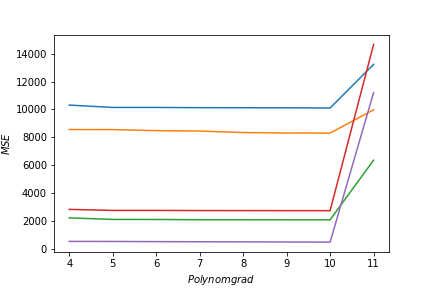
\includegraphics[width=100mm]{MSEE_OLS}
\caption{MSE OLS, brune stjerner er gjennomsnittet. for de forsjellige gradene }
\end{figure}
Verdien varierer mer med hvilken patch det vi har valgt isteden for, hvilken grad vi har valgt. Som vi vet skal jo MSE ha verdier som nærmer seg null. disse verdiene havner jo langt over 0. Så jeg vet egentlig ikke helt hva hvordan jeg skal tolke dette her.

\begin{figure}[H]
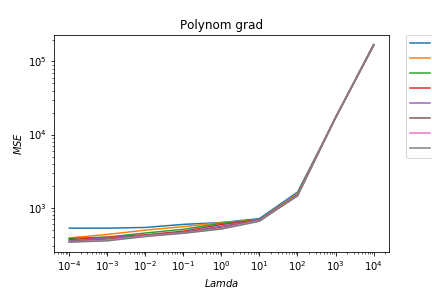
\includegraphics[width=100mm]{MSE(ERi)}
\caption{MSE av RIge av 5 forsjelige deler av ekte data som jeg valgte  }
\end{figure}
På Rige MSE figur 20  ser vi samme mønstret som vi har sett tidliger bare at vi har verdiene er mange ganger større verdien vi hadde på frankfungsjonen. Så lenge $\lambda$-ene holder seg lave så er de stabiel. Det er heller ikke stor varjasjon i gradene.
\begin{figure}[H]
\includegraphics[width=100mm]{MSE(ELi)}
\caption{MSE vs $\lambda$. Tatt gjennomsnitte av de 5 forsjelige delene, for hver $\lambda$ av ekte data som jeg valgte  }
\end{figure}
Lasso har også verdier som er sky høye. Den har samme oppfører seg likt med $\lambda$. Den stiger kraftig når $\lambda$ begyner å stige 
\subsection*{R2}

\begin{figure}[H]
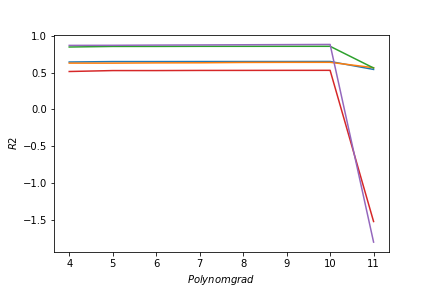
\includegraphics[width=100mm]{R2E_OLS}
\caption{R2 vs graden til x, y }
\end{figure}
Verdie er ikke noe bedre her. De er skyhøye. Vet ikke hvordan jeg skal tolke det uten om at $y_{i} - \widetilde{ y}$ den diferangsen må være ganske stor og at $y -\bar{y}$ må være liten.

\begin{figure}[H]
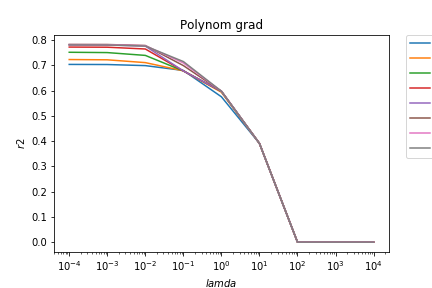
\includegraphics[width=100mm]{r2(ERi)}
\caption{R2 vs log($\lambda$), Gradene varier fra 4-11. Rige }
\end{figure}
Det er var jo ganske fasinerende å se at vi får en r2 verdi som faktisk er innefor en realistiske verider. De er jo ikke noe gode verdier. Det er ogsp ineresangt å se at når lambda blir stor så blir verdien  negativ.
\begin{figure}[H]
\includegraphics[width=100mm]{r2(ELi)}
\caption{R2 vs log($\lambda$), Gradene varier fra 4-11. Lasso }
\end{figure}
Det er er jo ganske fasinerde for har vi faktisk verdier som er gode r2 verdier figur24. $0.9999 + 0.000092=0.999992$. Den oppfører seg også likt som i frankfunksjonen  hvor verdien faller. Men holder seg gode.
\subsection*{Varianc}
\begin{figure}[H]
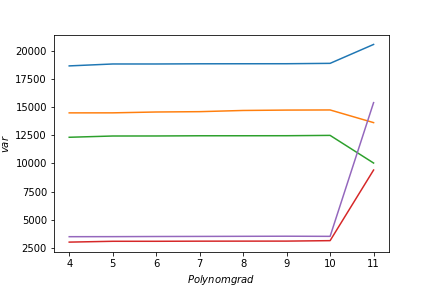
\includegraphics[width=100mm]{varE_OLS}
\caption{Varians vs gradenen til x, y, OLS }
\end{figure}
Sondig att variansen ikke varier??

\begin{figure}[H]
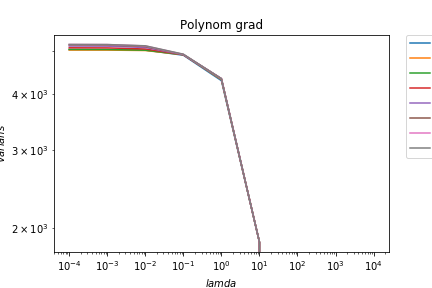
\includegraphics[width=100mm]{var(ERi)}
\caption{var vs log($\lambda$), Gradene varier fra 4-11. Med Rige }
\end{figure}
Følger samme mønstret som frankfunsjonen, Når $\lambda$ blir større synker variansen, men denne gangen noe savkere. 
\begin{figure}[H]
\includegraphics[width=100mm]{var(ELi)}
\caption{var vs log($\lambda$), Gradene varier fra 4-11,Med Lasso   }
\end{figure}
Følger samme mønstret som frankfunsjonen, Når $\lambda$ blir større synker variansen, men den har en helt ekstrem endring fra helle$10000 til 0,0000009$. Dette skjønner jeg faktisk. Dette kommer av at når $\lambda$ blir stor vel den nominer så mye av at alle verdien til z blir like og vi ender med null varians. Så meget lav varians er faktisk en dårlig ting. 
\subsection*{$Bias^2$}
\begin{figure}[H]
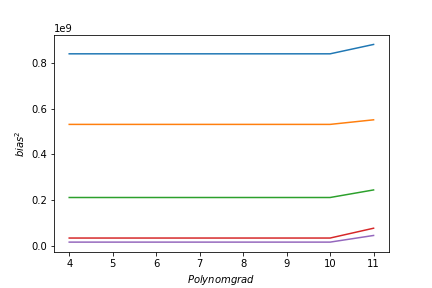
\includegraphics[width=100mm]{biasE_OLS}
\caption{Bias vs Graden($x^{g},y^{g}$), g=[4,11] }
\end{figure}
Veldig høye verdier her. Det varier noen i fra data sett til data sett.

\begin{figure}[H]
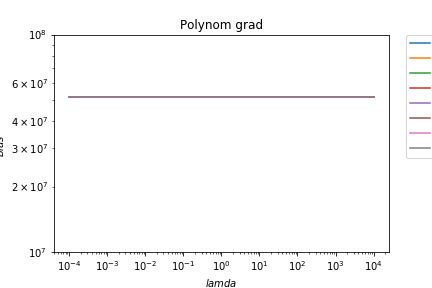
\includegraphics[width=100mm]{bias(ERi)}
\caption{Bias2 vs $\lambda$, Rige. gradene går fra 4 til 11  }
\end{figure}
Veldig høye verdier her
\begin{figure}[H]
\includegraphics[width=100mm]{bias(ELi)}
\caption{Bias2 vs $\lambda$, Lasso. gradene går fra 4 til 11   }
\end{figure}
Sotore verdier på biasen her også
\subsection*{Diskusjon}
Mye rare tall men at formen nogen lunde kommer frem er klart. Noen av tallen kan forklares, men jeg greer Heller ikke her å få MSE som stemmer med bias og varians. Vi får så klart ekstremt fosjellige verdier fra den vi har delen fra datan,men viser at vi kan gjenskape følelse av  den såkalte funksjonen til datan. Selv om vi bommer langt fra verdiene.
\section*{Diskusjon, data og frankfunksjon}
Det jeg vet ikke helt hvordan jeg skal tolke disse tallen de er altfor høye. og det er veldig merklig at r2 verdien for lasso og rige holder seg i det ommerået som er akseptabelt. Vi kan se fra 3d plottene i figuene 16-18 at det har likheter med den orginale delene. Men de er ganske langt fra orginalen. Det er da som man kan forvente at verdien ikke er helt er like som den funksjonen. 3d grafen er jo ikke like.
\\
Fra testen på frankfunksjon kan vi si lignet mer på den funksjonen
\section*{konklusjon}
Jeg tror jeg kan komme frem til en konkulsjon Rige er mer stabil iforhold til det jeg har gjort. Detter baserer jeg på den har gode verdier på frankfunksjonen, men også gode visuelle 3d plot. På ekte data har jo ridge nogenlunde likt 3d plot som ols og lasso men greie aksptable verdier på r2. Alle har syke verdier på real data. Men det virker som att det faktisk er mulig å kunne pruke denne metoden på for kunne spå z(x,y). Men jeg kan ikke konkluder så veldi mye med de verdien jeg har fåt På data delen. Noe jeg ikke skjønner hvorfor jeg ikke får til at $MSE=bias^{2} + var$\\
jeg tror jeg også kan konkludere med empirisk av studert rige og lasso av at det lav $\lambda $ som gir de beste verdien. Iverfall på de data delen jeg sett på og frankfunksjonen

\section*{hjelpemidler}
\url{<https://compphysics.github.io/MachineLearning/doc/web/course.htmll>}
\\

\url{<https://en.wikipedia.org/wiki/Bias–variance-tradeoff>}
\\
\url{<https://www.springer.com/gp/book/9780387848570f>}
\\
\url{<https://piazza.com/class/ji78s1cduul39a?cid=75>}
Mer på at jeg har brukt piatzza til løse oppgavene.
A high-bias, low-variance introduction to Machine Learning for physicists
Pankaj Mehta, Ching-Hao Wang, Alexandre G. R. Day, and Clint Richardson




\end{document}